\documentclass{article}
\usepackage{algorithm}
\usepackage{algpseudocodex}
\usepackage{graphicx}
\usepackage{amsmath}
\title{CSEP521 : Applied Algorithms: Homework 2}
\author{Karuna Sagar Krishna}

\begin{document}
    \maketitle

    \section*{Question 1}

    \subsection*{Idea}
    Breadth first search algorithm constructs the shortest path tree $T$. If there are edges in $G$ that are not present in $T$ then adding such an edge to $T$ will form a cycle in $T$. This is because all vertices in $T$ are connected and hence there already exists some path between the ends of this edge. By adding this edge to $T$, we now have two distinct paths between these ends forming a cycle. Further, we can claim that every non-tree edge forms a distinct cycle. In other words, if we have $k$ non-tree edges, then we have atleast $k$ cycles. And since $T$ can have exactly $n-1$ edges, so $k=m-(n-1)$.

    To output the cycle, we find the lowest common ancestor for the ends of the non-tree edge. This can done by keeping track of the levels and parents of each newly discovered vertex. Once we have the lowest common ancestor we need to output the path in right order.

    \subsection*{Algorithm}
        \begin{algorithm}[H]
            \begin{algorithmic}
                \Procedure{FindCycle}{$G$}
                    \For{$s \in G.Vertices$}
                        \If{$discovered[s] == false$}
                            \State $BFS(G, s)$
                        \EndIf
                    \EndFor

                    \If{$foundCycle$}
                        \State \Return $GetCycle(G, nonTreeEdge)$
                    \Else
                        \State \Return $\emptyset$
                    \EndIf
                \EndProcedure

                \Procedure{BFS}{$G, s$}
                    \State $discovered[s] = true$
                    \State $parent[s] = s$
                    \State $level[s] = 0$
                    \State $startingVertex[s] = s$
                    \Comment{we'll use this in question 4}
                    \State $queue.add(s)$

                    \While{$!queue.empty()$}
                        \State $u = queue.remove()$
                        \For{$(u,v) \in G.Edges$}
                            \If{$disovered[v] == false$}
                                \State $discovered[v] = true$
                                \State $parent[v] = u$
                                \State $level[v] = level[u]+1$
                                \State $startingVertex[v] = s$
                                \Comment{we'll use this in question 4}
                                \State $queue.add(v)$
                            \Else
                                \State $foundCycle = true$
                                \State $nonTreeEdge = (u,v)$
                            \EndIf
                        \EndFor
                    \EndWhile
                \EndProcedure

                \Procedure{GetCycle}{$G, f$}
                    \State $cycle = []$

                    \State $LowestCommonAncestor(f.u, f.v)$

                    \State $cycle.Add(f)$
                    \State $cycle.Add(pathV)$
                    \State $Reverse(pathU)$
                    \State $cycle.Add(pathU)$

                    \State \Return $cycle$
                \EndProcedure

                \Procedure{LowestCommonAncestor}{$u, v$}
                    \If{$level[u] > level[v]$}
                        \State $(u,v) = (v,u)$
                    \EndIf

                    \While{$level[v] > level[u]$}
                        \State $pathV.add((v, parent[v]))$
                        \State $v = parent[v]$
                    \EndWhile

                    \While{$u \neq v$}
                        \State $pathU.add((u, parent[u]))$
                        \State $u = parent[u]$

                        \State $pathV.add((v, parent[v]))$
                        \State $v = parent[v]$
                    \EndWhile

                    \State \Return $u$
                \EndProcedure
            \end{algorithmic}
        \end{algorithm}

    \subsection*{Correctness}
    As discussed in class, BFS finds the shortest path tree $T$ rooted at the starting vertex $s$. Note this is a spanning tree for the connected component containing $s$ and there cannot be a cycle across two different connected components.

    The BFS algorithm introduced in class has been modified to track the level and parent of each vertex. When a new vertex is discovered for the first time we record the parent as the vertex used to make this discovery and level is recorded as $1+$ the level of the parent vertex. We also track one non-tree edge which is used to return a cycle in $G$.

    Claim: The presence of non-tree edge indicates that there is a cycle in $G$. To prove this, when BFS algorithm finds that a vertex is already discovered, that edge is not part of the shortest path tree $T$. Consider one such non-tree edge $(u, v)$, since $T$ is a connected tree (within the connected component), there exists exactly one path $P$ between $u$ and $v$. And note, $(u, v) \notin P$. So, $P \cup (u, v)$ forms a cycle. Hence, $foundCycle$ correctly indicates presence of cycle in $G$. Also, each non-tree edge implies forms a distinct cycle, hence $k$ non-tree edges forms atleast $k$ distinct cycles.

    To output the found cycle in $G$, we need to find $P$ corresponding to the non-tree edge $(u, v)$. Note, the algorithm records one such non-tree edge in $nonTreeEdge = (u, v)$. Since BFS produces a rooted tree from the starting vertex, there is a common ancestor for $u$ and $v$. Say, $a$ is lowest common ancestor, then $P$ can be decomposed as path from $v$ to $a$ and path from $a$ to $u$. This decomposition can be easily constructed from the parent and level information we tracked during the BFS algorithm.

    \subsection*{Analysis}
    As proved in class, the BFS algorithm takes $O(n+m)$ time for $G$. This remains the same despite our modifications since our modifications are $O(1)$. This implies we can determine the presence of a cycle in $G$ in $O(n+m)$ time.

    To return a cycle, we find $P$ which takes atmost $O(m)$ time. This is because we navigate up the tree $T$ and we might visit all edges at worst case (think of $G$ to be a one big cycle). Overall, we need $O(n+m)+O(m) = O(n+m)$ for $FindCycle$ algorithm.

    \section*{Question 2}

    \subsection*{Idea}
    Clearly, merge sort technique cannot be used since that would take linear time. Since the lists of integers are sorted (assuming ascending order) and the question asks us to provide a $O(\log m + \log n)$ solution, it hints that at each step we somehow reduce the length of the lists by a factor of 2. We could compare the middle element of the two lists indicating the order of these middle elements in the hypothetically merged list. Based on the value of $k$ we can eliminate half of the input lists from our search space and we recursively solve this subproblem.
    
    \subsection*{Algorithm}
        \begin{algorithm}[H]
            \begin{algorithmic}
                \Procedure{FindKth}{$a, b, k$}
                    \State $m = len(a)$
                    \State $n = len(b)$
                    \If{$m == 0$}
                        \State \Return $b[k]$
                    \EndIf
                    \If{$n == 0$}
                        \State \Return $a[k]$
                    \EndIf
                    \If{$m == 1$}
                        \State $Insert(b, a[1])$
                        \State \Return $b[k]$
                    \EndIf
                    \If{$n == 1$}
                        \State $Insert(a, b[1])$
                        \State \Return $a[k]$
                    \EndIf
                    \If{$a[m/2] < b[n/2]$}
                        \If{$k < (m+n)/2$}
                            \State $FindKth(a, b[1..n/2], k)$
                        \Else
                            \State $FindKth(a[m/2..m], b, k-m/2)$
                        \EndIf
                    \Else
                        \If{$k < (m+n)/2$}
                            \State $FindKth(a[1..m/2], b, k)$
                        \Else
                            \State $FindKth(a, b[n/2..n], k-n/2)$
                        \EndIf
                    \EndIf
                \EndProcedure

                \Procedure{Insert}{$x, l$}
                    \State $n = len(x)$
                    \If{$n == 1$}
                        \If{$l < x[1]$}
                            \State \Return $l + x$
                        \Else
                            \State \Return $x + l$
                        \EndIf
                    \EndIf
                    \If{$l < x[n/2]$}
                        \State $Insert(x[0..n/2], l)$
                    \Else
                        \State $Insert(x[n/2..n], l)$
                    \EndIf
                \EndProcedure
            \end{algorithmic}
        \end{algorithm}

    \subsection*{Correctness}
    At each step of the algorithm, one half of the passed list is eliminated from search space and which half is eliminated depends on where the middle elements $a[m/2]$ and $b[n/2]$ reside in the merged list. Note, we don't compute this list in our algorithm, we only use it to argue the correctness. Consider, the below diagram illustrating this merged list and the positions of the middle elements. When $a[m/2] < b[n/2]$, the position of $a[m/2]$ is in the range $[m/2, (m+n)/2]$ because at a atleast $m/2$ elements are less than $a[m/2]$ and atmost $m/2 + n/2$ elements are less than $a[m/2]$. The position of $b[n/2]$ is in the range $[(m+n)/2, m+n/2]$ because atleast $m/2 + n/2$ elements are less than $b[n/2]$ and atleast $n/2$ elements are greater than $b[n/2]$ implying that atmost $(m+n)-n/2 = m+n/2$ elements are less than $b[n/2]$. Similar argument can be made when $a[m/2] > b[n/2]$ as shown in the diagram below.

    \begin{figure}[H]
        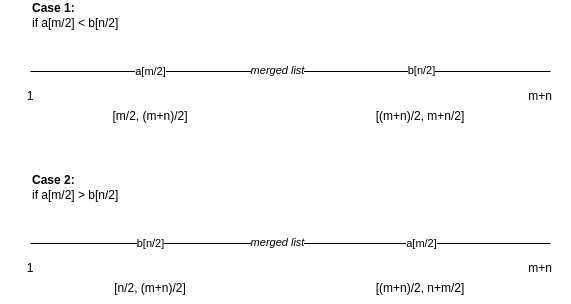
\includegraphics[width=1\textwidth]{findkth.png}
    \end{figure}

    During case 1, if $k < (m+n)/2$, then we can eliminate $b[n/2..n]$ from our search space as the kth element cannot be greater than $b[n/2]$ and recursively find the $k$ element.Otherwise, we can eliminate $a[0..m/2]$ since kth element cannot be less than $a[m/2]$ and recursively find the $k-m/2$ element. Similarly, we eliminate the appropriate half in case 2 and recursively find the kth element adjusting $k$ as needed for the subproblem.

    The recursive calls end when the number of elements in one of the lists reduce to a single element at which point we insert this single element into the other list using binary search technique. And clearly the kth element in single sorted list is $list[k]$.

    \subsection*{Analysis}
    The runtime of the $FindKth(a, b, k)$ algorithm can be expressed by the following recurrence.

    \begin{equation*}
        T(m, n) = 
        \begin{cases}
            T(m, n/2) + O(1) & \text{if we eliminate one half of b} \\
            T(m/2, n) + O(1) & \text{if we eliminate one half of a} \\
            log(m)           & \text{if n == 1} \\
            log(n)           & \text{if m == 1} \\
            O(1)             & \text{if m == 0 or n == 0}
        \end{cases}
    \end{equation*}

    This recurrence can be simplified as, at the end of $i$ steps, $T(m, n) = T(m/2^j, n/2^{i-j}) + i*O(1) : 0 \le j \le i$. This recurrence terminates when we no longer are able to halve the one of the list i.e. when one of the list contains a single element. Say first list reduces to a single element i.e. $m/2^j = 1 \implies j = \log m$, so the recurrence solves to:
    
    \begin{equation*}
        \begin{split}
            T(m, n) 
            & = T(1, n2^j/2^i) + i*O(1) \\
            & = T(1, nm/2^i) + i \\
            & = log(nm/2^i) + i \\
            & = log(nm) - log(2^i) + i \\
            & = log(nm) - i + i \\
            & = log(n) + log(m)
        \end{split}
    \end{equation*}

    In case, the second list reduces to a single element i.e. $n/2^{i-j} = 1 \implies i-j = \log n$, so the recurrence solves to:

    \begin{equation*}
        \begin{split}
            T(m, n) 
            & = T(m/2^j, 1) + i*O(1) \\
            & = T(m/2^{i-log n}, 1) + i \\
            & = T(m2^{log n}/2^i, 1) + i \\
            & = T(mn/2^i, 1) + i \\
            & = log(mn/2^i) + i \\
            & = log(mn) - log(2^i) + i \\
            & = log(mn) - i + i \\
            & = log(m) + log(n)
        \end{split}
    \end{equation*}

    Hence, the algorithm takes $O(\log m + \log n)$ time.

    \section*{Question 3}

    \subsection*{Idea}
    Using the union-find data structure, consider each variable $x_i$ to be a set element. We iterate over all the equality constraints $x_i = x_j$ and merge $x_i$ and $x_j$. Then we iterate over all disequality constraints $x_i \neq x_j$ and check if $x_i$ and $x_j$ belong to the same set. If they belong to same set, the constraints cannot be satisfied.
    
    \subsection*{Algorithm}
        \begin{algorithm}[H]
            \begin{algorithmic}
                \Procedure{CanSatisfyConstraints}{$constraints$}
                    \For{$constraint \in constraints$}
                        \If{$constraint.operator == "equals"$}
                            \State $(x_i, x_j) = constraint.operands$
                            \State $merge(x_i, x_j)$
                        \EndIf
                    \EndFor

                    \State $canSatisfy = true$
                    \For{$constraint \in constraints$}
                        \If{$constraint.operator == "not-equals"$}
                            \State $(x_i, x_j) = constraint.operands$
                            \If{$find(x_i) == find(x_j)$}
                                \State $canSatisfy = false$
                            \EndIf
                        \EndIf
                    \EndFor
                    \Return $canSatisfy$
                \EndProcedure
            \end{algorithmic}
        \end{algorithm}

    \subsection*{Correctness}
    The equals operation is transitive i.e. $(x_i = x_j) \land (x_j = x_k) \implies (x_i = x_k)$. This allows us to iterate over the equality constraints and merge the variables into a single set. In other words, at any point in time, all variables in a set are equal. Next, we iterate through the disequality constraints verifying it can be satisfied by ensuring the participating variables are in different sets. If all disequality constraints can be satisfied, then we can satisfy the problem.

    \subsection*{Analysis}
    As we proved in class, union and merge operations each operate in $O(\log n)$ time. We are given $m$ constraints, so in total the algorithm runs in $O(m \log n)$ time.

    \section*{Question 4}

    \subsection*{Idea}
    As hinted in the question, we can use the cut and cycle properties of MST trees to verify if the provided tree is MST. The edge $e$ whose weight was updated, can either belong to $T$ or not. If $e \in T$, then we verify the cut property on the cut formed by $T-\{e\}$. If $e$ has the minimum weight across the cut, we can say $T$ remains MST, else $T$ is not MST. If $e \notin T$, then we verify the cycle property on $T \cup \{e\}$; note, adding $e$ to $T$ forms exactly one cycle. If $e$ has the maximum weight among all the edge in the cycle in $T \cup \{e\}$, then $T$ remains MST, else $T$ is no longer MST.
    
    \subsection*{Algorithm}
        \begin{algorithm}[H]
            \begin{algorithmic}
                \Procedure{IsMST}{$G, T, e$}
                    \If{$e \in T.Edges$}
                        \State \Return $IsCutPropertySatisfied(G, T, e)$
                    \Else
                        \State \Return $IsCyclePropertySatisfied(G, T, e)$
                    \EndIf
                \EndProcedure

                \Procedure{IsCutPropertySatisfied}{$G, T, e$}
                    \For{$s \in T.Vertices$}
                        \If{$discovered[s] == false$}
                            \State $BFS(T-\{e\}, s)$
                        \EndIf
                    \EndFor

                    \State $satisified = true$
                    \For{$f \in G.Edges$}
                        \If{$startingVertex[f.u] \neq startingVertex[f.v]$}
                            \If{$w(f) < w(e)$}
                                \State $satisified = false$
                            \EndIf
                        \EndIf
                    \EndFor

                    \State \Return $satisfied$
                \EndProcedure

                \Procedure{IsCyclePropertySatisfied}{$G, T, e$}
                    \State $c = FindCycle(T \cup \{e\})$

                    \State $satisified = true$
                    \For{$f \in c$}
                        \If{$w(f) > w(e)$}
                            \State $satisfied = false$
                        \EndIf
                    \EndFor

                    \State \Return $satisfied$
                \EndProcedure
            \end{algorithmic}
        \end{algorithm}

    \subsection*{Correctness}
    To prove correctness, we need consider 2 cases - when $e \in T$ and $e \notin T$.

    When $e \in T$, we leverage the cut property for MST proved in class. The cut property states that edge with minimum weight across the cut should be part of all MST trees. Note, $T$ was MST before we updated the edge weight for $e$. Consider the cut formed by removing $e$ from $T$, so $T$ becomes disconnected with 2 connected components (2 connected trees). To identify the 2 connected components in $T-\{e\}$, we use a modified BFS algorithm on $T-\{e\}$ where we update the $startingVertex$ for each newly discovered nodes. Since, BFS algorithm discovers all the vertices in the connected component, $startingVertex[v]$ represents the label of connected component that $v$ belongs to. Further, note $T-\{e\}$ has exactly 2 connected components so $startingVertex[v]$ contains only 2 distinct values across all vertices. This helps us identify edges that go across the cut since the ends of such an edge would have to reside in different connected components.

    There could be multiple edges between the 2 connected components. The claim is - to ensure that $T$ is MST, we can only include only such edge and that edge should have the lowest weight among all the edges across the cut. It is clear that including more than one edge across cut will create a cycle. Adding the first edge will connect the 2 connected trees i.e. there is exactly one path between every 2 vertices. So when the second edge is added it will create a second path between the ends of this second edge leading to a cycle. So, we include only one edge across the cut. And this edge should have minimum weight, if not we can replace it with another edge across the cut with lower weight connecting the 2 components to form a MST (cut property). If such an edge is $e$ then $T$ remains MST, else it is no longer an MST.

    When $e \notin T$, we leverage the cycle property for MST proved in class. The cycle property states that edge with maximum weight in the cycle cannot be part of any MST. Note, $T$ was MST before we updated the edge weight for $e$. $T$ contains no cycles, but $T \cup \{e\}$ has exactly one cycle i.e. say, $e = (u,v)$ then $T$ contains exactly one path $P$ between $u$ and $v$, so $T \cup \{e\}$ contains exactly one cycle $c$. We then find the the edge in this cycle with maximum weight, say $f$. If $f \notin T$ then $f == e$ and applying cycle property we can say that $T$ remains MST. If $f \in T$, then $T$ cannot be MST as stated by cycle property. This is because we can remove $f$ from $T$ which leads to 2 connected components and there is some edge in cycle $\neq f$ that connects to the 2 connected components. This edge has lower weight than $f$ leading to connected tree with lower overall weight than $T$. Hence $T$ is not MST. Also note, that the edge with lower weight has to be $e$ since $(e \neq f) \land (e \notin T) \land (e \in c)$.

    \subsection*{Analysis}
    Running time of $IsMST(G, T, e)$ is maximum of $IsCutPropertySatisfied$ and $IsCyclePropertySatisfied$.

    $IsCutPropertySatisfied(G, T, e)$ run BFS on $T-\{e\}$ which has $n$ vertices and $(n-1)-1$ edges (a tree has $n-1$ edges). So, BFS on $T-\{e\}$ runs in $O(n+n-2) = O(n)$. We then iterate over all edges of $G$ in $O(m)$. Hence, the total running time of $IsCutPropertySatisfied(G, T, E)$ is $O(n) + O(m) = O(n+m)$. Note in $G$, $m >= n-1$ since $G$ is connected (which is because it has a MST), so our running time becomes $O(m)$.

    $IsCyclePropertySatisfied(G, T, e)$ runs FindCycle from Question 1 which takes $O(n+m)$ on $G$. But note, we run FindCycle on $T \cup \{e\}$ which has $(n-1)+1 = n$ edges leading to a running time of $O(n+n) = O(n)$. And then we iterate over all the edges in $c$ which could have a maximum of $m$ edges. Hence, the total running time of $IsCyclePropertySatisfied(G, T, e)$ is $O(n) + O(m) = O(n+m)$ and as mentioned above $m >= n-1$, so we have $O(m)$.

    Hence, $IsMST(G, T, e)$ runs in $O(m)$ time.

\end{document}
